\section{Grafi}
Un \textbf{grafo} è una struttura usata per rappresentare relazioni tra oggetti, i quali sono rappresentati da \textbf{nodi} (vertices), mentre le relazioni tra di essi sono rappresentate da \textbf{archi} (edges). È un concetto versatile abbastanza da poter rappresentare qualunque cosa possa essere messa in relazione, come per esempio una rete stradale che collega le città oppure gli stati di una FSM.\par
Diciamo inoltre \textbf{cammino} una sequenza di nodi collegati dagli archi e spesso i problemi trattano la ricerca del cammino \textbf{ottimo}, la cui definizione varia in base alla richiesta. Ciò implica la presenza di un qualche tipo di misura; chiamiamo intuitivamente \textbf{lunghezza} di un cammino il numero di archi attraversati in un percorso. Ci sono inoltre più tipi di grafo: \begin{itemize}
	\item \textbf{Grafo orientato}: Grafo i cui cammini sono orientati in una direzione. Presenta un nodo \textbf{sorgente} ed uno di \textbf{destinazione}. È possibile inoltre avere archi che ritornano sullo stesso nodo, ed in tal caso vale come passo.
	\item \textbf{Grafo non orientato}: Caso speciale del tipo precedente, i cammini possono andare in ambo le direzioni.
	\item \textbf{Grafo pesato}: Grafo i cui archi hanno associato un valore matematico, detto \textbf{peso}. Il costo totale è dato dalla somma dei valori degli archi attraversati.
\end{itemize}
\noindent Queste erano tutte definizioni intuitive, ma è necessario garantire formalità per poter lavorare con queste rappresentazioni. Definiamo formalmente un grafo come la coppia: \[G = (V,E)\]
\noindent Dove $V$ è l'\textbf{insieme dei nodi} ed $E$ rappresenta quello degli \textbf{archi}. In particolare, per i grafi orientati, quest'ultimo è una coppia ordinata di vertici: $E \subseteq V\times V$. In questo senso un grafo può essere visto anche come una relazione binaria sull’insieme dei vertici, connettendo la struttura con le relazioni e alle matrici. Per esempio, potremmo definire un grafo simmetrico grazie al concetto di relazione simmetrica e otterremmo la dimostrazione di un grafo non orientato.\par
Definiamo ora formalmente il concetto di cammino: una sequenza di nodi tali per cui per ogni coppia di nodi ci sia un arco che li connette, quindi: \[v_0, ..., v_n \text{ tale che } \forall i < n \land i\geq 0 (v_i, v_{i+1})\in E\]
\noindent In questi termini possiamo intendere la lunghezza di un cammino come la distanza fra due nodi, definita come il numero totale di nodi meno $1$. Un cammino può contenere nodi ripetuti; in particolare, se inizia e termina nello stesso nodo si parla di \textbf{ciclo}. Un grafo che contiene almeno un ciclo è detto \textbf{ciclico}, altrimenti è \textbf{aciclico}.\par
Generalmente, vale la regola che se un grafo ha lunghezza maggiore del suo numero di nodi distinti, avrà sicuramente almeno un cammino ciclico. Parliamo adesso di \textbf{grado} dei nodi; ne esistono due tipi: \begin{itemize}
	\item \textbf{Grado uscente}: Numero di archi che escono dal nodo, formalmente la cardinalità di insieme $v$ tale per cui la coppia $(u,v)$ appartiene ad $E$: \[outDeg(u) = |\{v | (u,v)\in E\}|\]
	\item \textbf{Grado entrante}: Numero di archi che entrano nel nodo, formalmente la cardinalità di insieme $u$ tale per cui la coppia $(u,v)$ appartiene ad $E$: \[inDeg(v) = |\{u | (u,v)\in E\}|\]
	\item \textbf{Grado totale}: Somma dei due valori precedenti: \[inDeg + outDeg\]
\end{itemize}
\noindent Altri concetti importanti sono il \textbf{diametro} di un grafo, che indica la massima distanza del cammino minimo tra due nodi, definita come: \[diam(G) = max(dst(u,v))\]
\noindent I \textbf{sottografi}, intuitivamente un insieme di nodi più piccolo o uguale ottenuto a partire da un altro grafo, definiti come: \[G' = (V', E') \text{ tale che } V'\subseteq V \land E'\subseteq E\]
\noindent I \textbf{grafi completi} vedono invece ogni coppia di nodi collegata da un arco, la cui definizione differisce in base all'orientazione: \[\text{Non orientato: } \frac{n(n-1)}{2}\quad\text{ Orientato: }n(n-1)\]
\begin{figure}[h]
	\centering
	\subcaptionbox{Grafo orientato}{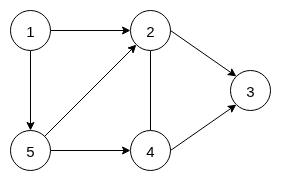
\includegraphics[width=0.3\linewidth]{Images/graphOriented.png}}
	\hfill
	\subcaptionbox{Grafo non orientato}{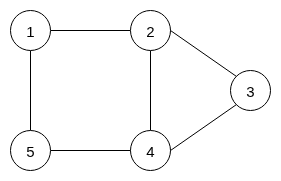
\includegraphics[width=0.3\linewidth]{Images/graphNoOrientation.png}}
	\hfill
	\subcaptionbox{Grafo pesato}{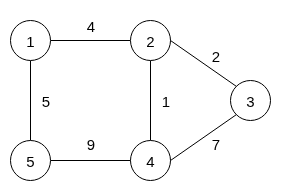
\includegraphics[width=0.3\linewidth]{Images/graphWeighted.png}}
\end{figure}
\noindent Esistono due tecniche principali per rappresentare i grafi in memoria: le \textbf{liste di adiacenza} e le \textbf{matrici di adiacenza}. Le prime utilizzano un array indicizzato sui nodi, dove ogni posizione contiene la lista dei nodi adiacenti, formalmente: \[Adj[u] = \{v|(u,v)\in E\}\]
\noindent La rappresentazione memorizza esclusivamente gli archi presenti nel grafo, risultando particolarmente efficiente in caso di grafi sparsi. Richiede uno spazio proporzionale alla somma di nodi e archi: \[\Theta(|V| + |E|), \text{ con abuso di notazione: } \Theta(V+E)\]
\noindent Nel caso di grafi pesati, ogni elemento della lista ha un campo per contenere il peso dell'arco.\par
\begin{figure}[h]
	\centering
	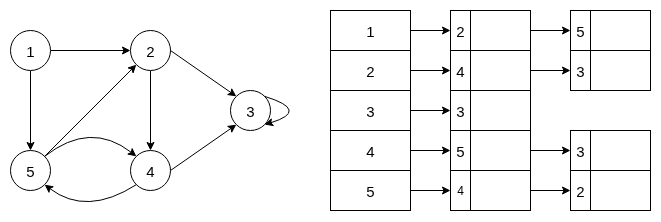
\includegraphics[width=1\linewidth]{Images/adjList.png}
	\caption{Lista di adiacenza}
\end{figure}
Le matrici di adiacenza, invece, utilizzano una matrice di dimensione $V\times V$ con valori booleani per segnalare le adiacenze per ogni nodo. Formalmente: \[G[i,j] = \begin{cases}
	1 & \text{Se esiste l'arco }(i,j)\\
	0 & \text{altrimenti}
\end{cases}\]
\noindent Nei grafi non orientati la matrice risulta \textbf{simmetrica} e lo spazio richiesto è $\Theta(V^2)$. È una rappresentazione inefficiente per grafi \textbf{sparsi} ($|E|$ è molto più piccolo di $|V|^2$), mentre per quelli completi risulta molto comoda. Per i grafi pesati, invece, al posto di valori booleani si utilizza direttamente il peso degli archi e l'assenza di un arco è segnalata con un valore sentinella, un infinito, oppure direttamente un NULL.
\begin{figure}[h]
	\centering
	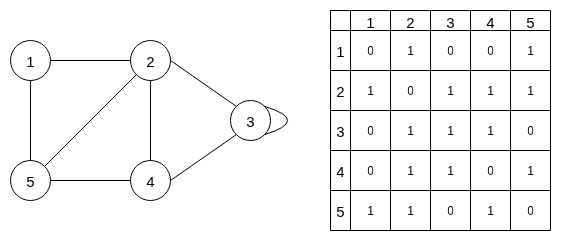
\includegraphics[width=0.8\linewidth]{Images/adjMatrix.png}
	\caption{Matrice di adiacenza}
\end{figure}
\noindent Facciamo ora un confronto fra le due rappresentazioni analizzando le modalità di calcolo del grado uscente. Con le liste bisogna contare ogni arco; nel caso pessimo abbiamo una complessità $\Theta(V)$, perché può essere che un nodo sia collegato a tutti gli altri. Alternativamente sarebbe possibile estendere la struttura dati con un campo size, garantendo un accesso a tempo costante.
\begin{algorithm}[h]
	\caption{outDeg((v,e), u)}
	\begin{algorithmic}[i]
		\Require $(v,e)$: coppia nodi-archi, $u$: Nodo il cui grado è calcolato
		\State $r\gets 0$
		\ForAll{$v\in Adj[u]$} \Comment{Per ogni nodo adiacente a u}
		\State $r\gets r+1$ \Comment{Aumenta il counter dei nodi adiacenti}
		\EndFor
		\State \textbf{return} $r$
	\end{algorithmic}
\end{algorithm}
\noindent Per il grado entrante bisogna scorrere l'intero grafo, oppure si può calcolare l'outDeg del grafo trasposto, ma costererebbe il doppio della memoria. Per le matrici di adiacenza invece si effettua la sommatoria della riga per il grado uscente e la sommatoria della colonna per quello entrante: \[outDeg = \sum_{j=1}^n G[i,j]\quad inDeg = \sum_{i=1}^n G[i,j]\]

%

\section{Visita in ampiezza}
Esistono molti algoritmi per l'esplorazione dei grafi; studieremo i due più utilizzati: la \textbf{visita in ampiezza} (BreadthFirstSearch o BFS) e la \textbf{visita in profondità} (DepthSearchFirst o DFS), cercando di rispondere a domande riguardo la struttura dei grafi, il cammino minimo e la raggiungibilità. Ci serviremo di un'importante campo per determinare lo stato dei singoli nodi. Diciamo che un nodo è: \begin{itemize}
	\item \textbf{Bianco} se non è stato esplorato.
	\item \textbf{Grigio} se è stato esplorato, ma non vi è stata effettuata alcuna operazione.
	\item \textbf{Nero} se è stato esplorato e sono state effettuate operazioni.
\end{itemize}
\noindent L'algoritmo BFS è uno dei più semplici per esplorare i grafi e viene utilizzato anche come base per procedure più complesse. Dato un grafo $G=(V,E)$ ed un nodo \textbf{sorgente} $s$, si esplorano gli archi del grafico per scoprire tutti i vertici raggiungibili da $s$.\par
Calcola inoltre la distanza fra di esso e ciascun nodo raggiungibile, dove la \textbf{distanza} da un vertice $v$ alla sorgente corrisponde al \textbf{cammino minimo} fra i due. Nella sua esecuzione genera un albero, detto \textbf{Albero BFS} (oppure BF-Tree) e funziona per grafi orientati e non orientati.
\begin{itemize}
	\item \textbf{Caso pessimo}: Temporale: $\Theta(|V|+|E|)$, Spaziale: $\Theta(|V|)$
	\item \textbf{Caso ottimo}: Temporale: $\Theta(|V|+|E|)$
	\item \textbf{Caso medio}: Temporale: $\Theta(|V|+|E|)$
\end{itemize}
\noindent Intuitivamente, una visita in ampiezza espande la frontiera dei vertici scoperti in maniera uniforme; partendo dalla sorgente $s$, scopre i suoi vicini a distanza $1$, poi a distanza $2$, e così via finché non trova tutti i vertici raggiungibili dalla sorgente.
\begin{algorithm}[h]
	\caption{BFS(G,s)}
	\begin{algorithmic}[i]
		\Require $G$: Grafo, $s$ Nodo sorgente
		\ForAll{$u\in V[G]$} \Comment{Per ogni nodo del grafo}
		\State $color[u]\gets white$ \Comment{Inizializza il nodo come non visitato}
		\State $d[u]\gets \infty$ \Comment{Distanza dalla sorgente del nodo}
		\State $\pi[u]\gets NIL$ \Comment{Predecessore nel BF-Tree}
		\EndFor
		\State
		\State $color[s]\gets gray$ \Comment{Nodo sorgente esplorato}
		\State $d[s]\gets 0$ \Comment{La distanza fra $s$ ed $s$ è $0$}
		\State $\pi[s]\gets NIL$ \Comment{La sorgente non ha predecessori}
		\State $Q\gets NIL$ \Comment{Coda fifo dei nodi grigi}
		\State enqueue($Q,s$)
		\State
		\While{$Q\neq NIL$} \Comment{Finché ci sono nodi grigi}
		\State $u\gets$ dequeue($Q$) \Comment{Prendi il primo nodo della coda}
		\ForAll{$v\in Adj[u]$} \Comment{Ogni nodo in lista di adiacenza di u}
		\If{$color[v] = white$} \Comment{Nodo non esplorato?}
		\State $color[v]\gets gray$ \Comment{Nodo ora esplorato}
		\State $d[v]\gets d[u]+1$ \Comment{La cui distanza è quella del precedente nodo ($u$) più uno}
		\State $\pi[v]\gets u$ \Comment{Predecessore è $u$}
		\State enqueue($Q,v$) \Comment{Nodo ora nella lista di quelli da elaborare}
		\EndIf
		\EndFor
		\State $color[u]\gets black$ \Comment{Il nodo è stato elaborato}
		\EndWhile
	\end{algorithmic}
\end{algorithm}

\noindent In necessità di ricavare i vertici di un cammino minimo da $s$ a $v$, supponendo sia già stata eseguita la BFS, è possibile utilizzare l'algoritmo \textbf{printPath} indicato alla pagina seguente.
\begin{algorithm}[h]
	\caption{printPath(G,s,v)}
	\begin{algorithmic}[i]
		\Require $G$: Grafo, $s,v$: Due nodi
		\If{$v = s$}
		\State print($s$)
		\ElsIf{$\pi[v] = NIL$}
		\State print(Nessun cammino da $s$ a $v$)
		\Else  
		\State printPath($G, s, \pi[v]$)
		\State print($v$)
		\EndIf
	\end{algorithmic}
\end{algorithm}

Analizziamo ora le varie sezioni dell'algoritmo per ricavarne il tempo di esecuzione. In primo luogo, i vertici sono colorati di bianco esclusivamente nell'inizializzazione e mai più dopo. La verifica di questo colore per ogni nodo nella lista di adiacenza garantisce che ogni nodo sia inserito e rimosso dalla coda al più una volta. Le operazioni di inserimento e cancellazione si eseguono in tempo costante, per un totale di $O(V)$.\par 
La somma delle lunghezze di tutte le liste di adiacenza è data da $\Theta(E)$, ed il tempo per visitarle tutte è pari a $O(V+E)$. In quanto il costo di inizializzazione è entro questo ordine di grandezza, possiamo concludere che il \textbf{tempo totale di esecuzione} per l'algoritmo BFS è di $O(V+E)$. Per la dimostrazione del funzionamento dell'algoritmo è necessario definire i seguenti lemmi: \begin{lemma}
	Sia il grafo $G=(V,E)$ e $s\in V$ un nodo arbitrario. Allora, per qualsiasi arco $(u,v)\in E$ si ha: \[\delta(s,v) \leq \delta(s,u)+1\]
\end{lemma}
\noindent Dunque per ogni coppia di nodi, il cammino minimo fra i nodi $s,v$ annotato come $\delta(s,v)$ non può essere più lungo di quello da $s$ ad $u$, seguito dall'arco $u,v$. Se $u$ non è raggiungibile, la distanza è infinita, mantenendo la validità della disuguaglianza. \begin{lemma}
	Sia $G=(V,E)$ un grafo e supponiamo che venga eseguita BFS a partire da un sorgente $s\in V$. Allora per ogni vertice $v\in V$, il valore di distanza $d[v]$ calcolato dall'algoritmo soddisfa sempre la seguente relazione, anche al termine della procedura: \[d[v] \geq \delta(s,v)\]
\end{lemma}
\noindent Intuitivamente, è possibile notare che il lemma è vero, poiché ogni valore assegnato a $d[v]$ è uguale al numero di archi di qualche cammino da $s$ a $v$. Per dimostrarlo formalmente, invece, è necessario ragionare per induzione sui passi eseguiti dalla funzione enqueue. Supponendo come ipotesi induttiva la relazione del lemma, abbiamo: \begin{itemize}
	\item \textbf{Caso base}: Inserimento della sorgente nella coda. L'ipotesi è vera, perché: \[d[s]=0=\delta(s,s);\quad d[v]=\infty\geq \delta(s,v)\quad\forall v\in V - \{s\}\]
	\item \textbf{Caso induttivo}: Consideriamo un vertice bianco $v$, scoperto nella visita a partire da un nodo $u$. L'ipotesi induttiva implica che $d[u]\geq \delta(s,u)$ e grazie al lemma precedente otteniamo: \begin{equation}
		\begin{split}
			d[v] &= d[u]+1\\
			&\geq \delta(s,u)+1\\
			&\geq \delta(s,v)
		\end{split}
	\end{equation}
\end{itemize}
\noindent Per dimostrare quest'ultima relazione è necessario capire meglio come opera la coda durante l'esecuzione della BFS. Il terzo lemma dice che in qualunque istante, la coda è sempre ordinata per una distanza non decrescente e contiene al più due valori: \begin{lemma}
	Supponiamo l'esecuzione di una BFS su un grafo $G=(V,E)$, con la coda $Q$ contenente i vertici $\left<v_1, v_2, ..., v_r \right>$, dove $v_1$ è il primo elemento della coda e $v_r$ l'ultimo. Allora: \[d[v_r]\leq d[v_1]+1 \text{ e } d[v_i]\leq d[v_{i+1}] \text{, con } i=1,2,...r-1\] 
\end{lemma}
\noindent Anche la dimostrazione di questo lemma avviene tramite induzione, ma questa volta sul numero di operazioni eseguite sulla coda. Inizialmente, quando questa contiene solo la sorgente, il lemma è banalmente valido, mentre per il passo induttivo è necessario provare che è valido dopo inserimento ed eliminazione di un nodo nella coda.\par
Per l'eliminazione di un nodo, quando la cima $v_1$ è eliminata, il successivo nodo $v_2$ diventa la nuova testa\footnote{Se $v_1$ era l'unico nodo, il lemma è banalmente valido.} e per ipotesi induttiva abbiamo: \[d[v_1] \leq d[v_2] \implies d[v_r]\leq d[v_1]+1\leq d[v_2]+1\]
\noindent Dunque rimuovere il primo elemento non rompe l'ordine e le restanti disuguaglianze rimangono inalterate. Il lemma è dimostrato con $v_2$ in cima alla coda.\par
Per l'inserimento di un nodo, invece, consideriamo la riga dove è invocato il metodo enqueue(); quando si inserisce il nodo in una coda, questo diventa $v_{r+1}$\footnote{Se la coda era vuota e questo è il primo nodo inserito, $r=1$ ed il lemma è vero banalmente.}. Attualmente il nodo in cima alla coda è $u = v_1$ e vale l'ipotesi per cui: \[d[u] \leq d[v_2];\quad d[v_r] \leq d[u]+1\]
\noindent Con una coda non vuota, gli si rimuove $u$ per elaborare la sua lista di adiacenza, ma così facendo, il nodo $v_2$ diventa la nuova cima $v_1$ della coda, facendo valere: \[d[u]\leq d[v_1] \implies d[v_{r+1}] = d[v] = d[u]+1\leq d[v_1]+1\]
\noindent Siccome $d[v_r]\leq d[u]+1$, abbiamo che $d[v_r]\leq d[u]+1 = d[v] = d[v_{r+1}]$ e le restanti disuguaglianze restano inalterate, facendo valere il lemma per l'inserimento di un nodo $v$.\newline

\noindent Adesso possiamo confermare la correttezza della visita in ampiezza. L'algoritmo calcola i cammini minimi e risolve il problema della raggiungibilità con il seguente teorema completo: \begin{teorema}
	\textbf{Correttezza della visita in ampiezza}\par
	\noindent Sia $G=(V,E)$ un grafo orientato o non orientato e supponiamo venga attuata una BFS a partire dal suo nodo sorgente $s\in V$. Allora, durante la sua esecuzione, BFS scopre tutti i nodi $v\in V$ raggiungibili dalla sorgente e, alla termine della sua esecuzione, viene calcolato il cammino minimo da $s$ a $v$ per ogni nodo del grafo. \[d[v]= \delta(s,v)\quad \forall v\in V\]
	\noindent Inoltre, per qualsiasi altro nodo $v \neq s$ raggiungibile da quest'ultimo, uno dei cammini minimi da $s$ a $v$ è un cammino minimo da $s$ a $\pi[v]$, seguito dall'arco $(\pi[v], v)$.
\end{teorema}
\noindent Per dimostrarlo, dividiamo i nodi per la distanza reale, definendo $V_k$ come l'insieme dei nodi a distanza $k$: \[V_k = \{v | \delta(s,v) = k\}\]
\noindent Dunque $V_0 = \{s\}$, $V_1 = $ nodi a livello $1$, e così via. Facendo induzione su $k$, dimostriamo che tutti nodi a questa distanza sono scoperti correttamente dalla BFS, dunque livello per livello. Per ogni nodo $v\in V_k$, esiste infatti un momento in cui: \begin{itemize}
	\item Il nodo $v$ è grigio.
	\item La distanza $k$ è assegnata a $d[v]$.
	\item Se il nodo corrente $v$ è diverso dalla sorgente $s$, il predecessore è $\pi[v] = u\in V_{k-1}$, quindi il nodo di livello superiore rimosso da dequeue().
	\item Il nodo $v$ è inserito in coda con enqueue().
\end{itemize}
\noindent Come passo base consideriamo $k=0$, quindi $V_0$, il livello della sorgente. In questo caso: \begin{itemize}
	\item $d[s] = 0 = k$, corretto.
	\item $s$ è grigio in quanto sta venendo elaborato, corretto.
	\item $s$ è attualmente in coda, corretto.
\end{itemize}
\noindent Come passo induttivo supponiamo vera l'ipotesi per $k-1$ prendendo un nodo $v\in V_k$. Per definizione di distanza minima, esiste un nodo a livello superiore $u\in V_{k-1}$ tale che esista un arco fra i due: $(u,v)\in E$. Per ipotesi induttiva: \begin{itemize}
	\item $u$ è scoperto correttamente.
	\item $d[u] = k-1$.
	\item $u$ è inserito in coda.
\end{itemize}
\noindent Quando $u$ è rimosso dalla coda per l'analisi della sua lista di adiacenza, scopro anche il nodo $v$ supposto all'inizio del passo, ottenendo $d[v] = d[u]+1 = k$, $\pi[v] = u$ e $v$ ottiene il colore grigio, dimostrando il teorema.\par
Inoltre, per l'ultimo lemma enunciato, possiamo confermare che $v$ non è stato precedentemente scoperto, perché avrebbe una distanza minore di $k$. Questo è impossibile perché $k$ è già il cammino minimo (quindi la distanza) tra la sorgente e il nodo.\newline

\noindent Il risultato di una BFS è un albero radicato nel nodo $s$ e se ci sono nodi non raggiunti, questi avranno distanza infinita da esso e non saranno parte dell'albero. Tuttavia, nulla vieta di eseguire un'altra procedura uguale sui nodi bianchi, creando nuovi alberi. Ciò consente di creare una \textbf{foresta} di alberi BFS.

%

\section{Visita in profondità}
L'algoritmo di \textbf{Visita in profondità} (DFS, Depth First Search) esplora gli archi uscenti dal vertice $v$ scoperto più recentemente e che ha ancora nodi non esplorati. La procedura continua finché non sono scoperti tutti i vertici raggiungibili da $v$. Fatto ciò, l'algoritmo sale di un livello per controllare eventuali altri nodi bianchi. Ripete il procedimento fino alla totale esplorazione del grafo. \begin{center}
	Caso pessimo temporale: $\Theta(|V| + |E|)$, caso pessimo spaziale: $\Theta(|V|)$
\end{center}
\noindent L'algoritmo forma un \textbf{sottografo dei predecessori} $G_\pi$ che può essere formato da più alberi, in quanto la visita può essere ripetuta da più sorgenti. Comprende sempre tutti i vertici e lo definiamo, insieme agli \textbf{archi d'albero}, come: \[G_\pi = (V, E_\pi);\quad E_\pi = \{(\pi[v], v) | v\in V \text{ e } \pi[v]\neq NIL\}\]
\noindent Oltre a creare la foresta, la DFS si serve di due \textbf{marcatempo}, per segnare il momento in cui un nodo viene scoperto $d[v]$ e l'istante in cui la visita completa l'ispezione della lista di adiacenze del nodo $f[v]$. Agevolano l'analisi del comportamento dell'algoritmo.
\begin{algorithm}[h]
	\caption{DFS(G)}
	\begin{algorithmic}[i]
		\Require $G$: Grafo
		\ForAll{$u\in V[G]$} \Comment{Inizializzazione del grafo}
		\State $color[u]\gets white,\quad \pi[u]\gets NIL$
		\EndFor
		\State $time\gets 0$ \Comment{Marcatempo globale per assegnare d[v], f[v]}
		\State
		\ForAll{$u\in V[G]$} \Comment{Visita ogni nodo bianco del grafo}
		\If{$color[u] = white$} \Comment{Se non è raggiunto, inizia una nuova visita DFS}
		\State $DFS\_Visit(G, u)$
		\EndIf
		\EndFor
	\end{algorithmic}
\end{algorithm}
\begin{algorithm}[h]
	\caption{DFS\_Visit(G, u)}
	\begin{algorithmic}[i]
		\Require $G$: Grafo, $u$: Nodo preso come sorgente
		\State $time\gets time+1$ \Comment{Aggiorno marcatempo}
		\State $d[u]\gets time,\quad color[u]\gets gray$ \Comment{Tempo in cui il nodo è scoperto}
		\State
		\ForAll{$v\in Adj[u]$} \Comment{Controlla tutti i suoi nodi figli}
		\If{$color[v] = white$} \Comment{Se non è esplorato, continua ad andare giù}
		\State $\pi[v]\gets u$
		\State $DFS\_Visit(G, v)$ \Comment{Ricorsione fa usare la stack per salvare i nodi}
		\EndIf
		\EndFor
		\State
		\State $time\gets time+1$
		\State $f[u]\gets time,\quad color[u]\gets black$ \Comment{Tempo in cui la visita è finita}
	\end{algorithmic}
\end{algorithm}

\noindent Prendiamo come esempio un grafo orientato di otto nodi. Scegliamo di invocare la procedura DFS considerando il nodo $s$ come la sorgente. Allora si controllerà ogni nodo nella sua lista di adiacenza fin quando non saranno stati esplorati tutti, segnando tempo di scoperta e tempo di conclusione esplorazione. Al termine della procedura avremo come risultato una foresta di due alberi; uno radicato in $s$ e l'altro in $t$.\par
La misura temporale dei nodi è molto importante, perché il tempo di elaborazione del nodo finale corrisponde esattamente al doppio del numero di nodi del grafo. Ciò accade perché si assegnano due misure temporali per nodo.
\begin{figure}[h]
	\centering
	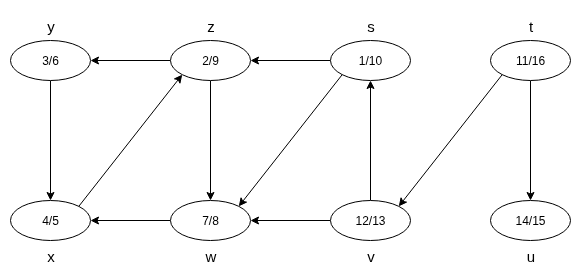
\includegraphics[width=1\linewidth]{Images/graph_DFS-example.png}
	\caption{Esempio di procedura DFS}
\end{figure}

\noindent Analizziamo ora la complessità dell'algoritmo: i primi due cicli for nel primo algoritmo usano un tempo $\Theta(V)$, poiché sono effettuati sull'intero insieme di nodi del grafo, escludendo la DFS\_Visit. Questa è invece chiamata una sola volta per ogni nodo bianco nelle liste di adiacenza, quindi $|Adj[v]|$ volte.\par
Siccome l'insieme delle liste di adiacenza compone quello degli archi e la visita è chiamata una sola volta per ogni nodo, confermiamo che DFS\_Visit ha complessità $\Theta(V+E)$; il tempo di esecuzione totale dell'algoritmo DFS è quindi $\Theta(V+E)$. Enunciamo ora alcuni teoremi importanti per questo algoritmo: \begin{teorema}
	\textbf{Teorema delle parentesi}\par
	\noindent In una qualsiasi visita in profondità di un grafo $G$ orientato o non orientato, per ogni coppia di vertici $u,v$ è soddisfatta esclusivamente una delle seguenti due condizioni: \begin{itemize}
		\item Gli intervalli $[d[u], f[u]]$ e $d[v], f[v]$ sono completamente disgiunti. I nodi non discendono l'uno dell'altro.
		\item L'intervallo $[d[u], f[u]]$ o $d[v], f[v]$ è interamente contenuto nell'altro, rendendo il primo nodo discendente del secondo.
	\end{itemize}
\end{teorema}
\noindent Per dimostrarlo, prendiamo la coppia di nodi $u,v$ e assumiamo, senza perdita di generalità, che valga la seconda relazione. Abbiamo quindi $d[u] < d[v]$ oppure $d[v] < d[u]$. Qui possiamo distinguere due casi: \begin{itemize}
	\item Se $f[u] < d[v]$ abbiamo due intervalli disgiunti, dimostrando la prima condizione del teorema.
	\item Se $d[v] < f[u]$ abbiamo un'intersezione tra gli insiemi, stando dentro la chiamata DFS\_Visit del nodo $u$. Ci troviamo quindi necessariamente in un sottointervallo i cui estremi sono $d[u], f[u]$, dimostrando che è interamente contenuto nel sovraintervallo.
\end{itemize}
\noindent Un'altra questione molto importante riguarda la possibilità di conoscere i discendenti a partire da un nodo sorgente. L'algoritmo DFS è capace di rispondere a questa domanda, servendosi del concetto dei nodi bianchi: \begin{teorema}
	\textbf{Teorema del cammino bianco}\par
	\noindent In una foresta di visita in profondità di un grafo $G$, orientato o non orientato, il vertice $v$ è discendente dal nodo $u$ se e solo se al tempo $d[u]$ in cui viene scoperto, il vertice $v$ può essere raggiunto dall'altro lungo un cammino formato esclusivamente da nodi bianchi.
\end{teorema}
\noindent Supponiamo infatti due nodi $u,v\in V$, di cui il secondo è discentente dal primo. Sia ora un terzo nodo $w$ nel cammino fra i due nella foresta. Se è bianco, il teorema è banalmente dimostrato perché l'intervallo di $w$ è interamente contenuto in quello di $u$.\par
In quanto discendente, il nodo $w$ è necessariamente visitato dopo il padre e sarà per forza bianco, perché l'unico modo per inizializzare il valore $d[w]$ è invocare DFS\_Visit, cosa che avviene solamente se il nodo è bianco. Difatti, prima di inizializzare $d[u]$, il nodo $w$ è bianco, e al tempo $d[u]$ esiste un cammino di nodi bianchi che comprende $w$.\par
Potremmo assumere ora per assurdo che $v$ non discenda da $u$ ma che abbia come predecessore $w$, discendente di $u$. Ne risulta la disuguaglianza: \[d[u] < d[w] < f[w] < f[u]\]
\noindent Allora al tempo $d[w]$ sto visitando i nodi della lista di adiacenza di $w$, nella quale è presente pure $v$, che inevitabilmente diventa discendente di $u$, dimostrando il teorema. Di nuovo.\newline

\noindent Durante una visita in profondità possono apparire diversi tipi di archi. Il loro studio consente di ottenere alcune importanti informazioni: \begin{itemize}
	\item \textbf{Archi d'albero} \textbf{T}: Archi che collegano un intervallo con un suo discendente.
	\item \textbf{Archi all'indietro} \textbf{B}: Archi che collegano un nodo al suo antenato.
	\item \textbf{Archi in avanti} \textbf{F}: Archi che collegano un intervallo con un discendente non diretto.
	\item \textbf{Archi trasversali} \textbf{C}: Archi che collegano due intervalli disgiunti.
\end{itemize}
\noindent In particolare, durante una visita in profondità è possibile riconoscere il tipo di arco in base al colore dei nodi: il bianco indica un arco d'albero, il grigio uno all'indietro, mentre il nero un arco in avanti o trasversale. Inoltre, se un grafo presenta archi all'indietro è sicuramente \textbf{ciclico}, perché, supponendo che la visita in profondità ne trovi uno, $v$ avrà colore grigio e $u$ sarà suo discendente. Esisterà di conseguenza un cammino tra i due nodi.\par
Supponiamo ora un grafo ciclico e prendiamo in esame un suo ciclo qualsiasi. Sia $u$ il suo primo nodo visitato in profondità e $v$ il predecessore di $u$ nel ciclo. Allora al tempo $d[v]$ tutti i nodi del ciclo tranne $u$ sono bianchi, rendendo il nodo $v$ raggiungibile a partire dall'altro con un cammino di soli nodi bianchi. In quanto tale, possiamo dire per il teorema del cammino bianco che $v$ discende da $u$ nella foresta e sarà visitato quando $u$ è grigio, dimostrando l'arco all'indietro.

%

\section{Ordinamento topologico}
Definiamo un \textbf{ordinamento topologico} di un grafo orientato aciclico (DAG) un ordinamento totale di tutti i suoi nodi, tale che, se $G$ contiene un arco $(u,v)$, allora $u$ appare prima di $v$. Possiamo immaginarlo come una distensione dei vertici lungo una linea orizzontale, in modo che tutti gli archi siano direzionati da sinistra a destra; con questi presupposti, non è un concetto applicabile a grafi ciclici. Intuitivamente, l'algoritmo sfrutta la visita in profondità e la stack di attivazione per salvare su di essa ogni nodo quando è colorato di nero. Eseguendo operazioni di pop, è possibile ottenere il grafo ordinato topologicamente.
\begin{algorithm}[h]
	\caption{topologicalSort(G)}
	\begin{algorithmic}[i]
		\Require $G$: Grafo orientato aciclico.
		\State Chiama $DFS(G)$ per calcolare $f[v]$ di ogni nodo del grafo
		\State Completata la visita di un nodo, esegui $push(v)$
		\State Elaborati tutti i nodi, esegui $pop()$ per ogni nodo in stack
	\end{algorithmic}
\end{algorithm}

\noindent È immediato capire che è possibile inserire i nodi ordinati in una qualunque struttura dati come una lista concatenata; basta semplicemente eseguire l'operazione di inserimento sul nodo rimosso dalla stack.
\begin{figure}[h]
	\centering
	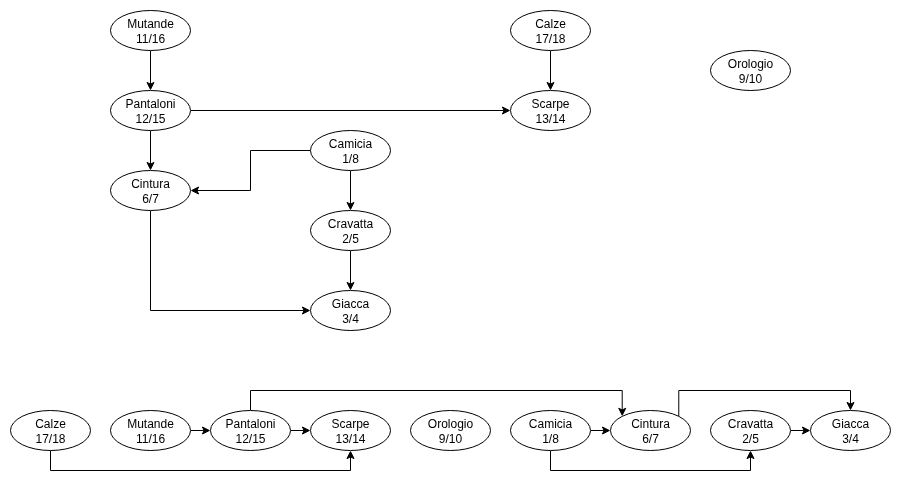
\includegraphics[width=1\linewidth]{Images/topologicalSort.png}
	\caption{Visualizzazione ordinamento topologico}
\end{figure}

\noindent L'algoritmo richiede un tempo $\Theta(V+E)$, perché è quello richiesto dalla visita in profondità. Inoltre, occorre un tempo costante $O(1)$ per rimuovere un totale di $|V|$ nodi dalla stack di attivazione. Per dimostrarlo, è in primo luogo necessario assicurarsi che il grafo passato per parametro sia aciclico grazie al seguente lemma: \begin{lemma}
	\textbf{Aciclicità di un grafo}\par
	\noindent Un grafo orientato $G$ è aciclico se e solo se in una sua visita in profondità non sono prodotti archi all'indietro.	
\end{lemma}
\noindent Supponiamo che eseguendo una DFS si produca un arco all'indietro $(u,v)$. Inevitabilmente, il nodo $v$ sarà un antenato di $u$ nella foresta DFS. Esisterà quindi un cammino nel grafo che va da $u$ a $v$ e l'arco all'indietro $(u,v)$ completa un ciclo. Potendo distinguere i tipi di grafo, possiamo enunciare il teorema: \begin{teorema}
	\textbf{Ordinamento topologico}\par
	\noindent L'algoritmo topologicalSort() produce un ordinamento topologico del grafo orientato aciclico che gli viene fornito in input.
\end{teorema}
\noindent Sappiamo che in questo algoritmo è invocata una visita in profondità su un grafo $G$ per calcolare il tempo di elaborazione di ogni suo nodo. Per dimostrare il teorema, è sufficiente provare che per una qualunque coppia di vertici distinti $u,v\in V$, se esiste un arco del grafo che va da $u$ a $v$, allora vale $f[v] < f[u]$.\par
Consideriamo quindi un arco qualsiasi; quando è visitato il vertice $v$ non può essere grigio, perché sarebbe antenato di $u$ e costituirebbe un arco all'indietro, rompendo il lemma precedente. Quindi, per qualunque arco, ci troviamo sicuramente in uno di questi due casi: \begin{itemize}
	\item Il nodo $v$ è bianco: $v$ è discendente di $u$ e vale $f[v] < f[u]$
	\item Il nodo $v$ è nero: la visita di $v$ è già stata completata e ha il valore $f[v]$ già impostato prima di $f[u]$. Dunque, certamente minore.
\end{itemize}
\noindent Un'altra comune applicazione della visita in profondità è la \textbf{scomposizione} di un grafo orientato nelle sue \textbf{componenti fortemente connesse} (SCC), il cui insieme è definito come il numero massimale di vertici $C\subseteq V$ tale che per ogni coppia di nodi $u,v\in C$, si ha che questi sono mutualmente raggiungibili.\par
In presenza di un grafo non orientato si potrebbe eseguire l'unione di tutti gli insiemi separati con componenti mutualmente raggiungibili, con il seguente algoritmo: \begin{algorithm}[h]
	\caption{ConnectedComponents(G)}
	\begin{algorithmic}[i]
		\Require $G$: Grafo aciclico non orientato
		\ForAll{$v\in V[G]$}
		\State makeSet(v)
		\EndFor
		\ForAll{$(u,v)\in E[G]$}
		\State union(u,v)
		\EndFor
	\end{algorithmic}
\end{algorithm}

\noindent Richiede un tempo lineare per l'esecuzione: $\Theta(V+E)$, tuttavia non è utilizzabile con grafi orientati, per i quali è richiesta una raggiungibilità \textbf{bidirezionale}. L'algoritmo per le componenti fortemente connesse, infatti, utilizza due visite in profondità; la prima per calcolare il tempo di elaborazione dei nodi del grafo, la seconda fa lo stesso, ma sul grafo trasposto $G^T$, definito come $G^T = (V,E^T)$, dove $E^T = \{(u,v):(v,u)\in E\}$, quindi con ogni arco inverso rispetto a quelli del principale grafo.\par
$G$ e $G^T$ hanno esattamente le stesse componenti fortemente connesse: due nodi sono raggiungibili l'uno dall'altro nel primo grafo se e solo se ciò vale anche nel trasposto. L'idea alla base dell'algoritmo deriva da una proprietà fondamentale del \textbf{grafo delle componenti} $SCC = (V^{SCC}, E^{SCC})$: supponiamo che un grafo abbia componenti fortemente connesse $C_1, ..., C_k$ e che l'insieme dei vertici $V^{SCC} = \{v_1, ..., v_k\}$ contiene un vertice $v_i$ per ogni $C_i$ del grafo. Esiste poi un arco $(v_i,v_j)\in E^{SCC}$ se $G$ contiene un arco orientato $(x,y)$ per qualche $x\in C_i$ e qualche $y\in C_j$.\par
Insomma, contraendo tutti gli archi i cui vertici incidenti sono all'interno della stessa componente fortemente connessa del grafo sicché rimanga un solo vertice, si ottiene il grafo $G^{SCC}$. Banalmente, raccogli le componenti mutualmente raggiungibili in un sottoinsieme e lo consideri componente fortemente connessa $C$. \begin{algorithm}[h]
	\caption{SCC(G)}
	\begin{algorithmic}[i]
		\Require $G$: Grafo aciclico orientato
		\State Chiama DFS(G) per calcolare $f[u]$ di ogni nodo $u$ del grafo
		\State Crea il grafo trasposto $G^T$
		\State Chiama DFS($G^T$) considerando i nodi in ordine decrescente rispetto a $f[u]$
		\State Ritorna i nodi di ogni albero della foresta DFS come una singola SCC
	\end{algorithmic}
\end{algorithm}

\noindent La procedura richiede un tempo lineare per il calcolo delle SCC, quindi $\Theta(V+E)$ e per dimostrarla è necessario enunciare i seguenti lemmi: \begin{lemma}
	\textbf{Distinzione delle componenti}\par
	\noindent Siano $C, C'$ due componenti fortemente connesse distinte in un grafo orientato $G$. Se $u,v\in C$ e $u',v'\in C'$, e supponendo ci sia un cammino che collega $u$ e $u'$, allora non può esistere anche un cammino da $v'$ a $v$ nello stesso grafo.
\end{lemma}
\noindent Il lemma è valido per la distinzione delle componenti, perché se esiste un cammino $v'\rightsquigarrow v$ nel grafo, allora esistono i cammini $u\rightsquigarrow u'\rightsquigarrow v'$ e $v'\rightsquigarrow v\rightsquigarrow u$, rendendo $u$ e $v$ raggiungibili mutualmente, contraddicendo l'ipotesi che $C$ e $C'$ siano SCC distinte.
\begin{lemma}
	\textbf{Tempo di elaborazione}\par
	\noindent Siano $C, C'$ due componenti fortemente connesse distinte in un grafo orientato. Supponiamo l'esistenza di un arco $(u,v)\in E$, dove $u\in C'$ e $v\in C$. Allora il tempo di fine visita di $C'$ è maggiore di $C$: $f(C') > f(C)$.
\end{lemma}
\noindent Per la dimostrazione è necessario considerare due casi, in base a quale SCC ha il nodo scoperto prima durante la visita DFS: \begin{itemize}
	\item Se $d(C') < d(C)$, diciamo $x$ il primo vertice scoperto in $C'$; quindi al tempo $d[x]$ tutti gli altri nodi sono bianchi e nel grafo esiste un cammino da $x$ a tutti gli altri composto da soli nodi bianchi, facendo valere il relativo teorema.\par
	In quanto tale, tutti i vertici di $C$ e $C'$ diventano discendenti di $x$ nell'albero di visita DFS e questo nodo avrà tempo di finitura massimo rispetto a tutti i suoi discendenti: $f[x] = f(C') > f(C)$.
	\item Se $d(C') > d(C)$, prendiamo $y$ primo vertice scoperto in $C$ per cui $d[y] = d(C)$, al cui tempo tutti i nodi in $C$ sono bianchi ed il grafo comprende un cammino da $y$ a tutti gli altri nodi in $C$, facendo valere il teorema del cammino bianco.\par
	In quanto tale, tutti i nodi di $C$ diventano discendenti di $y$ nell'albero della visita DFS e, per l'annidamento degli intervalli dei discendenti, vale $f[y] = f(C)$.\par
	Sappiamo inoltre che $d(C') < d(C) = d[y]$, al cui tempo tutti i vertici in $C'$ sono bianchi. Siccome esiste un arco da $C'$ a $C$, per rispettare la condizione che distingue le SCC, non esisterà un arco da $C$ a $C'$, rendendo tutti i vertici in quest'ultimo irraggiungibili da $y$. Dunque, al tempo $f[y]$ i vertici di $C'$ sono ancora bianchi, dimostrando che per qualunque vertice di $C'$ vale $f(C') > f(C)$.
\end{itemize}
\noindent Come conseguenza diretta, per garantire che le SCC rimangano distinte, il grafo trasposto non formerà nuovi archi per creare nuove componenti fortemente connesse. Abbiamo strumenti a sufficienza per la dimostrazione del teorema di questo algoritmo: \begin{teorema}
	\textbf{Componenti fortemente connesse}\par
	\noindent La procedura SCC() calcola correttamente le componenti fortemente connesse di un grafo orientato $G$.
\end{teorema}
\noindent La dimostrazione avviene per induzione sul numero di alberi creati dalla visita DFS sul grafo $G^T$. L'ipotesi è che i primi $k$ alberi formati siano componenti fortemente connesse. Quando $k=0$, banalmente, non avendo componenti, il teorema vale.\par
Nel passo induttivo supponiamo l'ipotesi e prendiamo in considerazione l'albero $(k+1)$-esimo e supponiamo che la sua radice sia il nodo $u$, che si trova nella SCC $C$. Per il funzionamento della visita DFS, al tempo di scoperta della radice, tutti gli altri nodi della SCC sono bianchi e formano un cammino nell'albero; inoltre, il tempo di completamento della radice sarà maggiore rispetto a quello di tutti gli altri nodi suoi discendenti.\par
Ogni arco in $G^T$ che esce da $C$ deve entrare in altre componenti già visitate, quindi nessun vertice appartenente a componenti diverse da $C$ è un discendente della radice $u$ nell'albero di visita DFS, provando che i vertici dell'albero DFS in $G^T$ formano esattamente una sola SCC, dimostrando il teorema.

%

\section{Alberi di copertura di costo minimo}
Spesso ci si trova davanti a problemi di ottimizzazione; nella teoria dei grafi si tratta il problema dell'\textbf{albero di copertura di costo minimo} (MST). Si parte da un grafo connesso non orientato, i cui archi hanno associato un valore, detto \textbf{peso}, che indica il costo richiesto per collegare due nodi. La soluzione di questo problema è un sottoinsieme aciclico del grafo di partenza che collega tutti i vertici, il cui peso totale è minimo.\par
Gli algoritmi trattati in questa sezione, \textbf{kruskal} e \textbf{prim}, sono avidi e utilizzano la stessa strategia di base applicata in modi differenti. Iniziamo definendo l'algoritmo per la creazione di un albero di copertura minimo \textbf{generic-MST()}, il quale prende in input un grafo connesso non orientato con una funzione per il peso. Costruisce l'albero di connessione minimo un arco alla volta, per poi ritornarlo al termine della sua esecuzione.\par
Questa procedura generica gestisce quindi un insieme $A$ di archi, assicurandosi che prima di ogni iterazione sia un sottoinsieme di qualche albero di connessione minimo.
\begin{algorithm}[h]
	\caption{generic-MST(G, w)}
	\begin{algorithmic}[i]
		\Require $G$: Grafo connesso non orientato, $w$: Valore del peso
		\State $A = \emptyset$
		\While{$A$ non è albero di connessione}
		\State Cerca un arco $(u,v)$ sicuro per $A$
		\State $A = A\cup \{(u,v)\}$
		\EndWhile
		\State return $A$
	\end{algorithmic}
\end{algorithm}
\noindent Per dimostrarne la correttezza abbiamo bisogno di definire alcune entità di base. Anzitutto, un \textbf{taglio} $(U, V-U)$ è una partizione dell'insieme dei nodi $V$, il quale sarà attraversato da alcuni archi, detti \textbf{archi del taglio}. Tra questi, quello con il peso minore è detto \textbf{arco sicuro} e sarà quello scelto per la costruzione dell'MST.
\begin{teorema}
	\textbf{Correttezza di generic-MST()}\par
	\noindent Sia $(u,v)$ un arco sicuro per un taglio $(U, V-U)$ in un grafo $G$, allora esiste un albero di copertura di costo minimo $T$ che contiene $(u,v)$.
\end{teorema}
\noindent Banalmente, se l'arco sicuro $(u,v)$ è all'interno di $T$, la tesi è dimostrata. Alternativamente, è possibile notare che, essendo il grafo connesso, esiste almeno un arco $(x,y)$ che attraversa il taglio. Se questo ha il costo minimo tra tutti gli archi del taglio disponibili, è quello sicuro, e sarà unito all'MST. Dunque: \[T' = T - \{(u,v) \cup (x,y)\}\]
\noindent Il grafo $T'$ è ancora un albero di copertura e il suo costo non è maggiore di quello di $T$. Pertanto $T'$ è un albero di copertura minimo che contiene $(u,v)$.\newline

\noindent Il primo algoritmo trattato è quello di \textbf{Kruskal}; trova un arco sicuro da aggiungere alla foresta in costruzione scegliendo l'arco dal peso minimo. Generalmente per la sua implementazione è usata una struttura dati per insiemi disgiunti; all'inizio saranno presenti vari set contenenti i vertici di un albero della foresta corrente. L'operazione di findSet(u) restituirà un rappresentante dell'insieme che contiene il nodo u, quindi per determinare se due vertici appartengono allo stesso insieme, si verifica se il risultato di findSet per entrambi è uguale. Per unire eventualmente gli alberi, si fa uso di union().\par
All'inizio dell'algoritmo è presente una fase di inizializzazione: si definisce la foresta vuota e si crea un insieme per ogni nodo del grafo. Si crea poi una lista di tutti gli archi del grafo e la si ordina con criterio monotono crescente rispetto al peso degli archi.\par
Dopodiché è presente un ciclo per la verifica di appartenenza ad uno stesso albero tramite findSet(). In caso affermativo, l'arco dei due nodi non può essere inserito perché è già dentro la foresta e viene quindi ignorato; alternativamente viene unito alla foresta e i nodi vengono fusi.
\begin{algorithm}[h]
	\caption{kruskal(G, w)}
	\begin{algorithmic}[i]
		\Require $G$: Grafo connesso, $w$: Peso dell'arco
		\State $A\gets\emptyset$
		\ForAll{$v\in V[G]$} $\text{ }makeset(v)$
		\State Crea una lista $L$ di tutti gli archi del grafo
		\State Ordina la lista in modo monotono non decrescente rispetto al peso $w$
		\EndFor
		\ForAll{$(u,v)\in L$ preso nell'ordine della lista}
		\If{$findSet(u)\neq findSet(v)$} \Comment{Se l'arco non è nella foresta, uniscilo}
		\State $A\gets A\cup \{(u,v)\}$
		\State $union(u,v)$
		\EndIf
		\EndFor
		\State \textbf{return} $A$
	\end{algorithmic}
\end{algorithm}

\noindent L'algoritmo di Kruskal non fa un taglio, data la richiesta di un grafo connesso abbiamo la garanzia che questo esiste, consentendoci di trovare un arco sicuro per qualche taglio che è garantito esista. L'insieme $A$ che ritorna la procedura è l'albero di copertura di costo minimo.\par
Il tempo di esecuzione di Kruskal dipende principalmente dalla struttura dati implementata per gli insiemi disgiunti. Consideriamo il costrutto ideale dato dalla \textbf{foresta di insiemi disgiunti} per ottenere il tempo asintoticamente minore rispetto ad altre implementazioni. L'inizializzazione richiede un tempo $O(1)$, creare una lista per ogni arco $O(V+E)$, ordinare gli archi $O(Elog(E))$, le operazioni del secondo ciclo for sono poi ripetute $O(E)$ volte. Assieme alle $|V|$ operazioni di makeSet(), le operazioni sugli insiemi disgiunti richiedono un tempo totale di: \[O((V+E)\alpha(V))\]
\noindent Con $\alpha$ funzione dalla crescita estremamente lenta. Essendo poi il grafo connesso, possiamo dire che $|E|\geq |V|-1$ e quindi le operazioni su insiemi disgiunti richiedono tempo $O(E\alpha(V))$. Da qui, osservando che $|E| < |V^2| \implies log|E| = O(log(V))$ possiamo concludere che il tempo di esecuzione totale per l'algoritmo di Kruskal è: \[O(Elog(E))\implies O(Elog(V))\]
\noindent Un altro algoritmo per il calcolo di MST è quello di \textbf{Prim}, la cui proprietà è che gli archi nell'insieme $A$ che costruisce in esecuzione formano sempre un albero singolo. Inizia infatti da un arbitrario nodo $r$, radice dell'albero, per poi andare a coprire tutti gli altri vertici passando sempre per gli archi dai pesi minimi.\par
Come input sono richiesti un grafo connesso $G$ e la radice dell'albero $r$. L'algoritmo è tipicamente implementato mantenendo una coda di priorità minima di tutti i vertici che non appartengono all'albero, basata su un attributo \textbf{key}, il peso minimo di un arco qualsiasi che collega $v$ a un nodo nell'albero. Si indica con $key[v]$. Inoltre, l'algoritmo mantiene implicitamente l'insieme $A$ come: \[A = \{(v, \pi[v]):v\in V - \{r\} - Q\}\]
\noindent Al termine dell'algoritmo, la coda creata è del tutto vuota ed è creato l'albero di connessione minimo tale che: \[A = \{(v,\pi[v]):v\in V-\{r\}\}\]
\begin{algorithm}[h]
	\caption{prim(G, w, r)}
	\begin{algorithmic}[i]
		\Require $G$: Grafo connesso, $w$: Peso dell'arco, $r$: Nodo radice
		\ForAll{$u\in V[G]$} \Comment{Ogni nodo a sé. No predecessore, distanze infinite.}
		\State $key[u]\gets \infty$, $\pi[u]\gets NIL$
		\EndFor
		\State $key[r]\gets 0$, $Q\gets \emptyset$
		\State
		\ForAll{$u\in V[G]$}
		\State $enqueue(Q, u)$
		\EndFor
		\State
		\While{$Q\neq\emptyset$}
		\State $u\gets extractMin(Q)$ \Comment{Prendo un nodo oltre il taglio}
		\ForAll{$v\in Adj[u]$}
		\If{$v\in Q \textbf{ AND } w(u,v) < key[v]$} \Comment{Se arco leggero è minore del corrente}
		\State $\pi[v]\gets u$, $key[v]\gets w(u,v)$ \Comment{Aggiorno i valori del nodo corrente}
		\State $reduceKey(Q, v, w(u,v))$ \Comment{Riduco la chiave perché trovato peso minore}
		\EndIf
		\EndFor
		\EndWhile
	\end{algorithmic}
\end{algorithm}

\noindent Il tempo di esecuzione di Prim, Come per Kruskal, dipende dalla struttura dati utilizzata per implementare la coda. Se $Q$ è un min-heap binario ci sarà richiesta una buildHeap(), di costo $O(V)$. Il corpo del while è eseguito $|V|$ volte e siccome ogni estrazione di minimo è eseguita in un tempo $O(log(V))$, il tempo totale per terminare il ciclo è $O(Vlog(V))$. Il ciclo for viene poi eseguito $|E|$ volte complessivamente e il test che verifica l'appartenenza alla coda $Q$ richiede tempo costante. Ogni chiamata a reduceKey() usa infine un tempo $O(log(V))$. Possiamo concludere che il tempo di esecuzione totale dell'algoritmo è: \[O(Vlog(V) + Elog(V)) = O(Elog(V))\]

%

\section{Cammini minimi a sorgente singola}
Il problema del \textbf{cammino minimo} è intuitivamente la ricerca di un percorso in un grafo da un nodo sorgente a una destinazione, il cui costo
totale, dato dalla somma dei pesi degli archi, è minimo. Formalmente, è richiesto un grafo orientato pesato $G = (V, E)$, la cui funzione peso descritta
da $w:E\to \mathbb{R}$ associa un valore ad ogni arco del grafo. Il peso di un cammino sarà dato dall'espressione: \[
	w(p) = \sum_{i=1}^{k} w(v_{i-1}, v_i)
\]
\noindent Mentre il peso di un cammino minimo $\delta(u, v)$ è definito come: \[
	\delta(u, v) = \begin{cases}
		min\{w(p) : u\rightsquigarrow v\} & \text{Se esiste un cammino tra i nodi}\\
		\infty & \text{Altrimenti}
	\end{cases}
\]
\noindent Dunque un cammino minimo da un nodo $u$ ad un vertice destinazione $v$ è definito come un cammino qualsiasi con peso $w(p) = \delta(u,v)$.
In particolare, questo percorso contiene anche i cammini minimi dalla sorgente a tutti i nodi intermedi per arrivare a $v$, grazie al seguente lemma:
\begin{lemma}
	\textbf{Sottocammini di cammini minimi}\par
	\noindent Dato un grafo orientato pesato $G$ con la relativa funzione del peso $w$, sia un cammino $p = \left<v_0, v_1, ..., v_k \right>$ quello
	minimo da $v_0$ a $v_k$. Consideriamo due valori $i,j$ compresi tra $0$ e $k$ tali da definire il percorso $p_{ij} = \left<v_i, v_{i+1}, ..., v_j \right>$.
	Quest'ultimo è un sottocammino di $p$ ed è anche il percorso minimo dal nodo $v_i$ al vertice $v_j$.
\end{lemma}

\noindent Per il corretto funzionamento degli algoritmi trattati in questa sezione, è necessario rispettare alcune condizioni per garantire la risolubilità
del problema preso in esame. Per esempio, supponiamo un grafo i cui pesi possono essere negativi; sarebbe possibile attraversare all'infinito l'arco con
tale valore per ridurre il costo del cammino. Ciò rimuove ogni significato della ricerca, e per questa ragione l'algoritmo di Dijkstra contempla
esclusivamente grafi pesati con valori non negativi.\par
Espandiamo il discorso considerando i cicli positivi: i grafi non possono contenere nemmeno questi, perché eliminandoli dal cammino si ottiene un
percorso con la stessa sorgente e destinazione con un peso più piccolo. Gli unici cicli contemplati sono quelli il cui attraversamento è a costo zero,
i quali si possono direttamente rimuovere dal grafo in quanto ininfluenti.\newline

\noindent La \textbf{rappresentazione} dei cammini minimi è simile a quella usata per gli alberi BFS. Dato un grafo definiamo un predecessore $\pi[v]$
che può essere un altro nodo o il valore NIL. È impostato in modo tale per cui sia possibile ripercorrere la catena dei predecessori, ritornando
appunto il cammino minimo tramite la procedura \textbf{printPath()}. Inoltre, grazie al lemma dei sottocammini, sappiamo che è possibile usare il
metodo per ritornare anche i sottocammini minimi. In ogni caso, il prodotto della funzione sarà un \textbf{albero di cammini minimi}, il quale conterrà
i percorsi dalla sorgente alla destinazione definiti minimi in base al peso degli archi.\par
Gli algoritmi della sezione usano la tecnica del \textbf{rilassamento}: la verifica dell'esistenza di un percorso migliore per la destinazione. Per
ogni vertice del grafo è mantenuto un valore $d[v]$ detto \textbf{stima del cammino minimo}, il quale è un limite superiore per il peso di un cammino
minimo dalla sorgente alla destinazione. Per eseguire calcoli corretti, è necessaria la seguente inizializzazione:
\begin{algorithm}[h]
	\caption{initializeSingleSource(G, s)}
	\begin{algorithmic}[i]
		\Require $G$: Grafo orientato pesato, $s$: Nodo sorgente
		\ForAll{$v\in V[G]$}
		\State $d[v]\gets \infty$
		\State $\pi[v]\gets \text{NIL}$
		\EndFor
		\State $d[s] = 0$
	\end{algorithmic}
\end{algorithm}

\noindent Questa procedura, essendo eseguita per ogni nodo del grafo, richiede un tempo di esecuzione $\Theta(V)$. Segue il rilassamento degli archi
grazie alla procedura \textbf{relax()}, eseguita in tempo $O(1)$:
\begin{algorithm}[h]
	\caption{relax(u, v, w)}
	\begin{algorithmic}[i]
		\Require $u$: Sorgente, $v$: Destinazione, $w$: Peso
		\If{$d[v] > d[u] + w(u,v)$} \Comment{Se è trovato un percorso migliore}
		\State $d[v]\gets d[u] + w(u,v)$ \Comment{Questa diventa la stima del cammino minimo}
		\State $\pi[v]\gets u$
		\EndIf
	\end{algorithmic}
\end{algorithm}

\noindent Il processo di rilassamento continua fino a quando non è più possibile rilassare gli archi; in tal caso è stato trovato il cammino minimo
dalla sorgente alla destinazione.\par
Il primo algoritmo discusso della sezione è quello di \textbf{Dijkstra}, il quale, eseguito su un grafo orientato pesato i cui costi degli
archi sono tutti non negativi, consente di trovare il cammino minimo da un nodo sorgente $s$ ad una destinazione $v$ e a tutti i nodi intermedi $u_i$
del percorso scelto secondo una strategia avida. Mantiene inoltre un insieme $S$ su vertici i cui pesi finali dei cammini minimi sono già stati
determinati; l'algoritmo seleziona infatti ripetutamente il vertice $u\in V - S$ con la stima minima; lo aggiunge a $S$ e rilassa tutti gli archi
uscenti dal nodo.
\begin{algorithm}[h]
	\caption{dijkstra(G, w, s)}
	\begin{algorithmic}[i]
		\Require $G$: Grafo pesato orientato, $w$: Peso non negativo, $s$: Sorgente
		\State initializeSingleSource(G, s)
		\State $S\gets \emptyset$
		\State $Q\gets \emptyset$
		\State
		\ForAll{$u\in V[G]$} \Comment{Inserisci ogni nodo nella coda}
		\State enqueue(Q, u)
		\EndFor
		\State
		\While{$Q\neq \emptyset$} \Comment{Finché la coda non è vuota}
		\State $u\gets$ extractMin(Q) \Comment{Estrai il nodo corrente}
		\State $S\gets S\cup {u}$ \Comment{Aggiungilo all'insieme}
		\ForAll{$v\in Adj[u]$} \Comment{Rilassa ogni arco nella sua lista di adiacenza}
		\State relax(u, v, w)
		\If{relax() diminuisce il valore $d[v]$} \Comment{Se trovato un cammino migliore}
		\State reduceKey(Q, v, d[v]) \Comment{Riduci la chiave della coda}
		\EndIf
		\EndFor
		\EndWhile
	\end{algorithmic}
\end{algorithm}

\noindent A seguito dell'inizializzazione della rappresentazione dei nodi $O(V)$, della coda e dell'insieme, si inseriscono tutti i nodi del grafo
nella coda $O(V)$, dalla quale ne sarà estratto uno alla volta, ad ogni iterazione del ciclo while, per un totale di $|V|$ volte.
Al suo interno si unisce il nodo estratto nell'insieme $S$ e si rilassano tutti gli archi da esso uscenti aggiornando la stima $d[u]$ e il predecessore
$\pi[v]$ se è trovato un cammino meno costoso. Quando ciò accade, si fa una chiamata alla funzione reduceKey() per aggiornare la coda. Ciò accade un 
totale di $|E|$ volte, quindi per ogni arco del grafo.\par
La complessità dell'algoritmo di Dijkstra dipende tuttavia anche dalla struttura dati utilizzata per la sua implementazione e quindi ragionare sulle
procedure di estrazione del minimo e riduzione chiave. In particolare: \begin{itemize}
	\item \textbf{Heap}: extractMin() e reduceKey() richiedono entrambe un tempo $log(n)$, facendo risultare come tempo totale di esecuzione: $(V+E)log(n)$.
	Si tratta dell'implementazione migliore per i grafi sparsi.
	\item \textbf{Liste ordinate}: extractMin() usa tempo costante, mentre reduceKey() costa $O(V)$. Dunque il tempo totale è di $O(V+VE)$.
	\item \textbf{Liste non ordinate}: extractMin() costa $V$ e reduceKey() $E$. La miglior opzione per i grafi completi ha quindi tempo di esecuzione
	totale $O(V^2 + E)$.
\end{itemize}
\noindent Come già menzionato, Dijkstra non funziona con grafi i cui pesi possono essere anche negativi, perché data la sua proprietà greedy, ovvero che
estrarre il nodo con stima minima garantisce che quella sia già definitiva, dipende dalla non negatività dei pesi. Con un arco negativo, un nodo già
estratto dalla coda e inserito nell'insieme potrebbe vedere la sua stima migliorata in seguito, ma non è possibile rivisitarlo.\par
Per contemplare i cicli negativi possiamo introdurre il secondo algoritmo: \textbf{Bellman-Ford}, che consente di trovare la soluzione al problema del
cammino minimo da singola sorgente anche in presenza di cicli negativi. Dato un grafo orientato pesato con un nodo sorgente e un peso, restituisce un
valore booleano che indica se esiste un ciclo negativo raggiungibile dalla sorgente. In tal caso, ritorna false, indicando che il problema non ha una
soluzione; altrimenti ritorna true insieme ai cammini minimi coi relativi pesi.
\begin{algorithm}[h]
	\caption{bellman-ford(G, w, s)}
	\begin{algorithmic}[i]
		\Require $G$: Grafo orientato pesato, $w$: Peso, $s$: Sorgente
		\State initializeSingleSource(G, s)
		\For{$i\gets 1$ to $|V[G]|-1$}
		\ForAll{$(u,v)\in E[G]$}
		\State relax(u, v, w)
		\EndFor
		\EndFor
		\State
		\ForAll{$(u,v)\in E[G]$} \Comment{Controlla se rimangono archi rilassabili}
		\If{$d[v] > d[u]+w(u,v)$} \Comment{Se sì, non c'è soluzione}
		\State \textbf{return} false
		\EndIf
		\EndFor
		\State \textbf{return} true
	\end{algorithmic}
\end{algorithm}

\noindent Dopo l'inizializzazione, l'algoritmo effettua un totale di $|V|-1$ passaggi sugli archi del grafo, ognuna corrispondente ad ogni iterazione
del primo ciclo for per il rilassamento di ogni arco. Il secondo ciclo for controlla l'esistenza di cicli negativi, ed in tal caso ritorna false.\par
Per confermare la correttezza dell'algoritmo è necessario in primo luogo dimostrare che in assenza di cicli di peso negativo, calcola correttamente i
pesi dei cammini minimi per ogni vertice raggiungibile dalla sorgente. Consideriamo un qualunque nodo $v$ raggiungibile dalla sorgente e indichiamo con
$p = \left<v_0, v_1, ..., v_k \right>$ il cammino minimo aciclico da $s$ a $v=v_k$.\par
Sicuramente il cammino avrà al più $|V|-1$ archi, quindi $k \leq |V|-1$. Ognuna delle iterazioni del ciclo for rilassa tutti gli $|E|$ archi. In quanto
comprende tutti i nodi all'interno del percorso, è capace di ritornare i cammini minimi per ognuno di loro a partire dalla sorgente. Inoltre, come
corollario, abbiamo la sicurezza che esiste un cammino tra due nodi $s, v$ se e solo se l'algoritmo termina con una stima $d[v] < \infty$.\newline

\noindent Supponiamo ora per assurdo che l'algoritmo ritorni un valore true anche in presenza di cicli di peso negativo. In tal caso, significa che per
ogni arco $(u,v)$ vale la condizione $d[v] \leq d[u] + w(u,v)$. Applicando questa disuguaglianza ad ogni arco del ciclo, otteniamo: \[
	\sum_{i=0} d[u_i] \leq \sum_{i=0} d[u_i] + \sum_{i=0} w(u_i, u_{i+1}) \implies 0 \leq \sum_{i=0} w(u_i, u_{i+1})
\]
\noindent Tuttavia ciò contraddice l'ipotesi che il ciclo sia negativo, perché risulta che sia maggiore o uguale di zero, provando il corretto
funzionamento dell'algoritmo di Bellman-Ford. Infine, lo studio della complessità risulta estremamente semplice, poiché è evidente come le operazioni
nei due cicli for siano eseguire prima su ogni nodo $O(V)$ e poi su ogni arco $O(E)$, dando come tempo di esecuzione totale $O(V\times E)$.\newline

\noindent Un ultimo algoritmo per il calcolo del cammino minimo a sorgente singola è quello di \textbf{dagShortestPath()}, il quale sfrutta il fatto
che in un grafo orientato aciclico esista sempre un ordinamento topologico. Ciò garantisce che quando si rilassa un arco, la stima $d[u]$ è già quella
definitiva, perché nessun arco potrà tornare su $u$.\par
Per ipotesi il grafo è aciclico ed è quindi possibile lavorare anche con pesi dal valore negativo. Richiede un'inizializzazione, un ordinamento
topologico tramite topologicalSort() e un rilassamento degli archi visitando il grafo ordinato. Sfruttando la struttura del dag, ottiene una complessità
temporale di $O(V+E)$.
\begin{algorithm}[h]
	\caption{dagShortestPath(G, w, s)}
	\begin{algorithmic}[i]
		\Require $G$: Grafo orientato aciclico, $w$: Peso, $s$: Sorgente
		\State initializeSingleSource(G, s)
		\State topologicalSort(G)
		\State
		\ForAll{$u\in V[G]$ ordinato}
		\ForAll{$v\in Adj[u]$}
		\State relax(u, v, w)
		\EndFor
		\EndFor
	\end{algorithmic}
\end{algorithm}

%

\section{Cammini minimi a sorgente multipla}
Floyd-Warshall, Johnson

\begin{comment}
--- Risoluzione del problema del cammino minimo per ogni coppia di nodi (a sorgente multipla)
Banalmente sarebbe possibile ripetere per ogni nodo la soluzione del cammino minimo a sorgente singola vista in precedenza. Dovremmo usare Bellman-ford ma avendo complessità VE e dovendolo ripetere V volte, avremmo V^2E.

Bisogna abbassare la complessità con alcune tecniche.
Anzitutto bisogna capire come rappresentare il problema. Usiamo la seguente notazione:
	- D_i: Vettore che comprende i costi dei cammini minimi
	- \pi_i: Vettore che comprende i predecessori
	- D_{i,j}: Costo del cammino minimo da i a j
	- \pi_{i,j}: Predecessore del nodo j nel cammino minimo da i a j
	
Per rappresentare la soluzione useremo quindi due vettori:
	- D = {D_1, D_2, ..., D_n} // Matrice dei cammini minimi
	- \Pi = {\pi_1, \pi_2, ..., \pi_n} // Matrice dei predecessori per i cammini minimi
Matrice perché array bidimensionali, capito? Possiamo rappresentare il problema con una matrice. Bisogna calcolare queste matrici, quindi.

// Proviamo ad applicare la soluzione oberosa discussa prima tramite bellman-ford
all_pairs_sp(G, w)
	D^0\gets init(G, w) // Inizializza ogni riga ponendo tutti gli elementi sulla diagonale a 0 e nel resto delle posizioni +\infty
	\For{l\gets 1 to |V[G]|-1} // Per ogni istanza del problema, quindi |V|-1 volte
		D^l\gets extend_sp(D^{l-1}, w) // extend shortest path, va a rilassare tutti gli archi relativi all'istanza corrente del problema
	
	D^{|V[G]|}\gets extend_st(D^{|V[G]|-1}, w)
	if D^{|V[G]|}\neq D^{|V[G]|-1} // Check per controllare se è stato sbagliato qualcosa nell'estensione della shortest path
		return false

// A partire dalla destinazione facciamo il rilassamento degli archi
extend_sp(D, w)
	n\gets rown[D] // Scopriamo la dimensione della matrice quadrata
	let D' be matrix n*n
	
	for i\gets 1 to n // Per ogni sorgente rilassa tutti gli archi. Sto aggiornando la distanza minima dal nodo di destinazione // i è la sorgente
		for j\gets 1 to n // j è la destinazione
			D'_{ij}\gets \infty // La distanza stimata iniziale dal nodo i a quello j è infinita. Va aggiornata tramite esplorazione grafo.
			
			for k\gets 1 to n // Per ogni possibile sorgente verso j
				D'_{ij}\gets min(D_{ij}, D_{ik}+w_{kj}) // facciamo il rilassamento verso l'arco kj, confrontando la minima distanza corrente con quella che otterresti passando dal nodo k attraverso l'arco kj di costo w_{kj}. Se è minore di D_{ij}, lo aggiorna.
	return D'
				
Quando w_{kj} non è un arco bisogna dare un peso che non causa problemi. Quindi il valore neutro per il minimo: \infty

Complessità di questo algoritmo: per p volte eseguiamo la shortest path. Ha tre cicli for eseguiti V volte. La all pairs ha un altro ciclo for eseguito V volte. Gesù, è O(V^4). Inoltre, se guardi alla struttura di extend_sp si può notare che è praticamente uguale a quella dell'algoritmo di moltiplicazione delle matrici, solo posto in un'algebra diversa, chiamata minPlus.
	Fondamentalmente è richiesta l'inizializzazione ad una matrice identità (quella con la diagonale principale a 0, le altre posizioni a infinito) sulla quale è possibile eseguire operazioni di somma e ricerca del minimo, allo stesso modo in cui si fanno quelle di somma e moltiplicazione. Valgono anche le stesse proprietà. Stiamo praticamente calcolando una potenza di w: w^4. C'è un modo per fare meno schifo?
	
Per ora, il prodotto di matrici ha complessità V^3; facendolo V volte otteniamo V^4. Si potrebbe parallelizzare l'algoritmo e poi rimettere insieme i pezzi successivamente, introducendo un fattore logaritmico e ottenendo una complessità V^3log(n).
Un'altra idea è l'algoritmo di floyd_warshall

// Algoritmo dinamico
floyd_warshall(w)
	D_{ij}^k // costo del cammino minimo da i a j che usa solo nodi di {1 ... k} come nodi intermedi
	
	n\gets rows[w]
	D^0\gets w // Matrice iniziale è quella dei pesi di w.
	
	for k\gets 1 to n
		for i \gets 1 to n // Calcoliamo la matrice di k supponendo di avere già disponibile quella di k-1
			for j\gets i to n
				D_{ij}^k\gets min(D_{ij}^{k-1}, D_{ik}^{k-1} + D_{kj}^{k-1}) // What the actual fuck, sta prendendo un cammino minore???
				
St'algoritmo ha complessità V^3. Costruiamo soluzioni vincolate, rendendo sempre più deboli i vincoli fin quando non arriviamo alla soluzione dei quali è priva.
Si può fare ancora meglio? Dipende dal caso, ma sì.
	Questo nuovo algoritmo funziona bene su grafi sparsi, ma male su quelli completi. Sul ragionamento di prima, se abbiamo tutti i pesi non negativi potremmo usare Dijkstra per ogni sorgente, ottenendo una complessità di V(V+E)logV = V^2logV + VElogV.
	Se il grafo è sparso, allora otteniamo V^2logV, sicuramente meglio di floyd-warshall. Se invece avessimo grafo sparso con pesi negativi? Johnson dice: trasformiamo i pesi del grafo in modo da non avere valori negativi?
	
La modalità per ottenere questa cosa è definire una funzione di potenziale. Definisce un nuovo costo che somma il costo base con la differenza dell'arco negativo
Sia h:V\to R. \hat{w}(u,v) = w(u,v) + h(u) - h(v)

Prendiamo dunque un cammino v_0, v_1, ..., v_n. Quanto vale \hat{w}(v_0, ..., v_n)?
\hat{w}(v_0, ..., v_n) &= \hat{w}(v_0, v_1) + \hat{w}(v_1, v_2) + ... + \hat{w}(v_{n-1}, v_n)\\
	&= w(v_0, v_1) + h(v_0) - h(v_1) + w(v_1, v_2) + h(v_1) - h(v_2) + ... + w(v_{n-1}, v_n) + h(v_{n-1}) - h(v_n)
	
Notare che fra tutti gli elementi si annullano h(v_1), h(v_2) e in generale tutte le h eccezion fatta per v_0 e v_n. Dall'espressione risulta quindi: \[\sum w(v_i, v_{i+1}) + h(v_0) - h(v_n) = w(v_0, ..., v_n) + h(v_0) - h(v_n)\]
\noindent Il costo nuovo è quindi uguale al costo vecchio sommato alla differenza tra gli estremi, facendo dipendere da essi il costo totale. Ciò non cambia la semantica del grafo, facendo valere la soluzione con Dijkstra.

Se ora trovassimo una funzione h per la quale Johnson mantiene i cammini minimi anche per grafi completi, abbiamo trovato un algoritmo migliore sempre di floyd_warshall.
	Supponiamo un grafo G e creiamo un supernodo collegato ad ogni nodo di G con peso 0. Usa bellman ford per calcolare i cammini minimi dal supernodo. Sia quindi d la funzione distanza minima. Sia inoltre h \Delta= d. Usa la funzione di distanza come la h definita prima quindi.
	
Complessità dell'algoritmo: VE + VElog(V), quindi bellman ford più l'algoritmo di prima.
	La complessità generale asintotica è VElog(V), mentre su grafi sparsi è V^2log(V). Come funziona?
	
\forall(u,v)\in E[G] abbiamo che d[v] \leq d[u] + w(u,v). L'arco non è rilassabile. Il peso nuovo non è negativo.
0 &\leq d[u] + w(u,v) - d[v]
	&= w(u,v) + d[u] - d[v] \equiv \hat{w}(u,v)
\end{comment}

%

\section{Flusso massimo}
Ford-Fulkerson, Karp